% !TeX root = ../main.tex
\chapter{模型构成}\label{ch4}

深度模型只不过是复杂的张量计算,最终可以用线性代数和数学分析分解为标准数学运算。多年来,该领域开发了大量语义清晰的高级模块以及由这些模块组合而来的复杂模型,这些模型已被证明在特定应用领域非常有效。

经验证据和理论结果表明,更深的架构(即长映射组合)可以获得更好的表现。正如我们在 \ref{sec3.4} 节中看到的,由于\keyterm{梯度消失},训练这样的模型具有挑战性,而多项重要技术贡献缓解了这个问题。

\section{层的概念}\label{sec4.1}

我们将那些被设计出来并通过经验认定为通用且高效的标准复杂复合张量操作称为\keyterm{层}。这些层通常包含可训练参数,并且对于设计和描述大型深度模型来说,它们提供了一个便捷的粒度级别。这个术语来源于简单多层神经网络,尽管现代模型可能采用此类模块的复杂图形形式,并包括多个并行路径。

\begin{figure}[h]
    \centering
    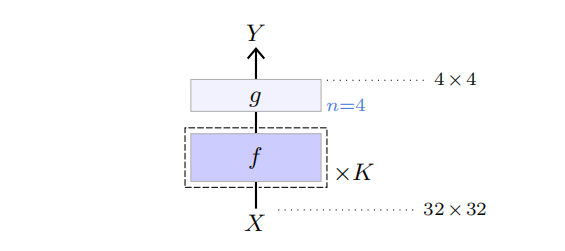
\includegraphics[width=0.9\textwidth]{fig/fig4.0.png}
\end{figure}

在接下来的几页中,我将遵循上面所示模型绘制的约定:

\begin{itemize}
    \item 算子/层被绘制为框,
    \item 深色表示嵌入了可训练的参数,
    \item 没有默认值的元参数用蓝色字添加在右侧,
    \item 带有乘法因子的虚线外框表示一组层按顺序复制,每个层都有自己的一组可训练参数(如果有的话),
    \item 在某些情况下,当输出维度与输入维度不同时,会在右侧标明。
\end{itemize}

此外,具有复杂内部结构的层会用高度更高的框来表示。

\section{线性层}\label{sec4.2}

就计算和参数数量而言,最重要的模块是\keyterm{线性层}。它们得益于数十年来在矩阵运算算法和芯片设计方面的研究与工程进步。

请注意,在深度学习中,``线性''这一术语通常不恰当地指代\keyterm{仿射运算},即一个线性表达式和一个常数偏置之和。

\subsubsection*{全连接层}

最基本的线性层是\keyterm{全连接层},由大小为 $D' \times D$ 的可训练权重矩阵 $W$ 和维度为 $D'$ 的偏置向量 $b$ 参数化。它实现了泛化到任意张量形状的仿射变换,其中补充的维度被解释为向量索引。形式上,给定维度为 $D_1 \times \dots \times D_K \times D$ 的输入 $X$,它计算出维度为 $D_1 \times \dots \times D_K \times D'$ 的输出 $Y$,其中
\begin{align*}
    \forall d_1,\dots,d_K&,\\
    Y[d_1&,\dots,d_K] = WX[d_1,\dots,d_K]+b
\end{align*}
虽然乍看之下,这种仿射运算似乎仅限于旋转、对称和平移等几何变换,但实际上它能做的远不止这些。特别是,用于降维或信号过滤的投影,而且,从点积作为相似性度量的角度来看,矩阵-向量乘积可以解释为计算输入向量所编码的查询与矩阵行所编码的键之间的匹配得分。

正如我们在 \ref{sec3.3} 节中看到的,梯度下降从\keyterm{参数的随机初始化}开始。如果这一操作做得过于简单,如 \ref{sec3.4} 节所示,网络可能会遭受激活和梯度爆炸或消失的影响 \citep{glorot10a}。深度学习框架实现了初始化方法,特别是按照输入的维度来缩放随机参数,以保持激活的方差恒定并防止病态行为。

\subsubsection*{卷积层}

线性层可以将任意形状的张量通过重塑成向量的方式作为输入,只要它具有正确数量的系数即可。然而,这样的层不太适合处理大型张量,因为参数数量和操作数量与输入和输出维度的乘积成正比。例如,要处理一个大小为 $256 \times 256$ 的 RGB 图像作为输入并计算相同大小的结果,将需要大约 $4 \times 10^{10}$ 个参数和乘法运算。

除了这些实际问题之外,大多数高维信号都是强结构化的。例如,图像在平移、缩放和某些对称性方面表现出短期相关性和统计平稳性。这并没有反映在全连接层的\keyterm{归纳偏置}中,它完全忽略了信号结构。

为了利用这些规律,首选的工具是\keyterm{卷积层}。卷积层同样是仿射的,但它局部处理时间序列或二维信号,并在各处使用相同的操作符。

\keyterm{一维卷积}主要由三个\keyterm{元参数}定义:内核大小 $K$、输入通道数 $D$、输出通道数 $D'$,以及仿射映射 $\phi(\cdot;w):\mathbb{R}^{D \times K} \to \mathbb{R}^{D' \times 1}$ 的可训练参数 $w$。

它可以处理任何大小为 $D \times T$ 且 $T \ge K$ 的张量 $X$,并将 $\phi(\cdot;w)$ 应用于 $X$ 的每个大小为 $D \times K$ 的子张量,将结果存储在大小为 $D' \times (T-K+1)$ 的张量 $Y$ 中,如图 \ref{fig4.1}(左半部分)所示。

\newpage

\begin{figure}[h]
    \centering
    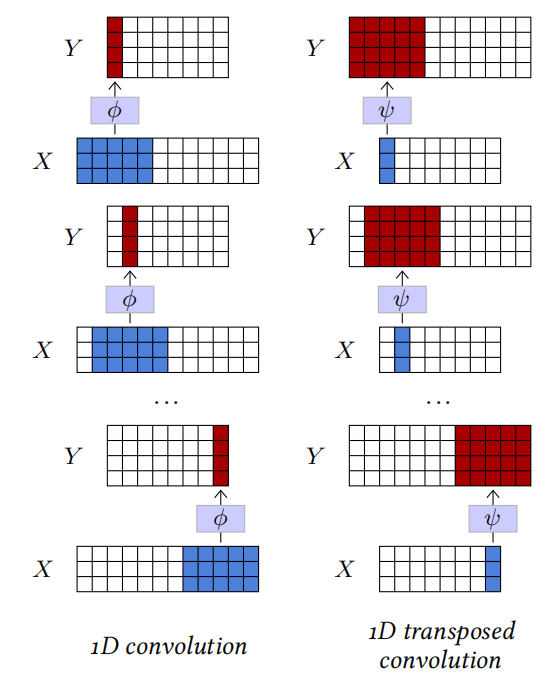
\includegraphics[width=0.9\textwidth]{fig/fig4.1.png}
    \caption[一维卷积]{一维卷积(左)接受 $D \times T$ 张量 $X$ 作为输入,将相同的仿射映射 $\phi(\cdot;w)$ 应用于形状为 $D \times K$ 的每个子张量,并将生成的 $D' \times 1$ 张量存储到 $Y$ 中。一维转置卷积(右)接受 $D \times T$ 张量作为输入,将相同的仿射映射 $\phi(\cdot;w)$ 应用于每个形状为 $D \times 1$ 的子张量,并对偏移后的 $D' \times K$ 结果张量求和。两者都可以处理不同大小的输入。}
    \label{fig4.1}
\end{figure}

\keyterm{二维卷积}与之类似,但具有 $K \times L$ 大小的内核,并接受 $D \times H \times W$ 大小的张量作为输入(参见图 \ref{fig4.2},左半部分)。

\begin{figure}[h]
    \centering
    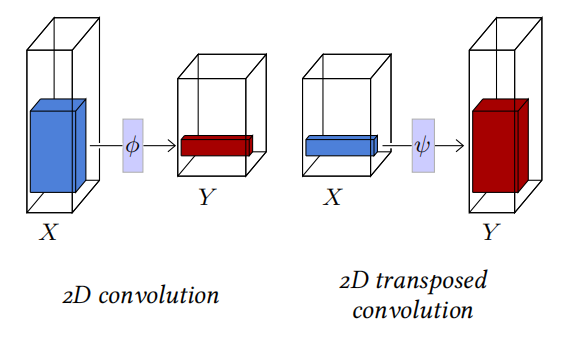
\includegraphics[width=0.9\textwidth]{fig/fig4.2.png}
    \caption[二维卷积]{二维卷积(左)接受 $D \times H \times W$ 张量 $X$ 作为输入,将相同的仿射映射 $\phi(\cdot;w)$ 应用于形状为 $D \times K \times L$ 的每个子张量,并将生成的 $D' \times 1 \times 1$ 张量存储到 $Y$ 中。二维 转置卷积(右)接受 $D \times H \times W$ 张量作为输入,将相同的仿射映射 $\phi(\cdot;w)$ 应用于每个形状为 $D \times 1 \times 1$ 的子张量,并对偏移后的 $D' \times K \times L$ 结果张量求和得到 $Y$。}
    \label{fig4.2}
\end{figure}



这两种操作的可训练参数都是 $\phi$ 的参数,可以分别将其设想为大小为 $D \times K$ 或 $D \times K \times L$ 的 $D'$ 个\keyterm{过滤器},以及一个维度为 $D'$ 的\keyterm{偏置向量}。

这样的层对平移是\keyterm{等变}的,这意味着如果输入信号被平移,输出也会以类似的方式变换。当处理其分布对于平移不变的信号时,此属性会产生理想的\keyterm{归纳偏差}。

卷积层还接受三个额外的\keyterm{元参数},如图 \ref{fig4.3} 所示:

\begin{itemize}
    \item \keyterm{填充}指定在处理输入张量之前应在输入张量周围添加多少个零系数,特别是在内核大小大于 $1$ 时维持张量尺寸。其默认值为 $0$。
    \item \keyterm{步幅}指定在处理输入时使用的步长,允许通过使用大步长以几何方式减小输出大小。其默认值为 $1$。
    \item \keyterm{膨胀}指定局部仿射操作符的过滤器系数之间的索引计数。其默认值为 $1$,更大的值对应于在系数之间插入零,这会增加过滤器/内核的大小,同时保持可训练参数数量不变。
\end{itemize}

\begin{figure}
    \centering
    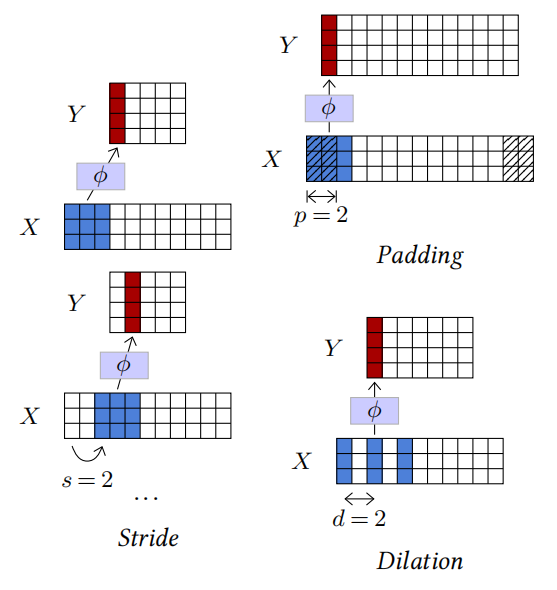
\includegraphics[width=0.9\textwidth]{fig/fig4.3.png}
    \caption[步长、填充和膨胀]{除了内核大小和输入/输出通道数之外,卷积还接受三个元参数:步长 $s$(左)在经过输入张量时调节步长,填充 $p$(右上)指定在处理输入张量之前在输入张量周围添加多少个零元素,膨胀 $d$(右下)参数化过滤器系数之间的索引计数。}
    \label{fig4.3}
\end{figure}

除了通道数之外,卷积的输出通常小于其输入。在没有填充或膨胀的一维情况下,如果输入的大小为 $T$,内核的大小为 $K$,步幅为 $S$,则输出的大小为 $T' = (T - K)/S + 1$。

\newpage

给定由卷积层计算的激活,或某个位置上所有通道的值向量,它所依赖的输入信号部分称为其\keyterm{感受野}(见图 \ref{fig4.4})。与 $D \times H \times W$ 激活张量的单个通道对应的 $H \times W$ 子张量之一称为\keyterm{激活图}。

\begin{figure}
    \centering
    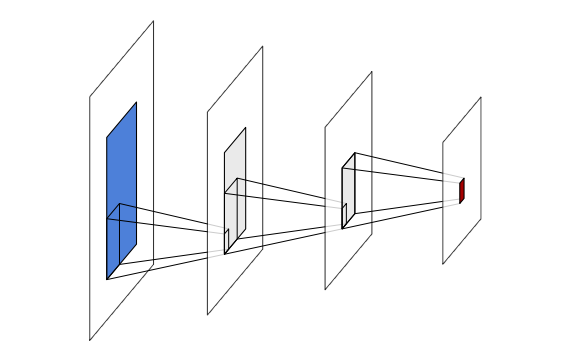
\includegraphics[width=0.9\textwidth]{fig/fig4.4.png}
    \caption[感受野]{给定一系列卷积层(这里为红色)中的激活,其\keyterm{感受野}是输入信号(蓝色)中调节其值的区域。每个中间卷积层大约按照核的宽度和高度增加该区域的宽度和高度。}
    \label{fig4.4}
\end{figure}

卷积用于重新组合信息,通常是为了减少表示的空间大小,以换取更多数量的通道,从而转化为更丰富的局部表示。它们可以实现微分算子,例如边缘检测器或模板匹配机制。一系列这样的层也可以视为一种组合和分层表示 \citep{arxiv-1311.2901},或者作为一个扩散过程,其中信息在穿过层时可以通过内核大小的一半进行传输。

逆运算是\keyterm{转置卷积},也由局部仿射算子组成,由与卷积类似的元和可训练参数定义,例如,在一维情况下,它将一个仿射映射 $\phi(\cdot;w):R^{D \times 1} \to R^{D' \times K}$ 应用于输入的每个 $D \times 1$ 子张量,并将偏移后的 $D' \times K$ 结果张量求和以计算其输出。这样的操作符增加了信号的尺寸,直观上可以理解为一个合成过程(见图 \ref{fig4.1} 和图 \ref{fig4.2} 的右半部分)。

一系列卷积层是将大维度信号(如图像或声音样本)映射到低维张量的常用架构。例如,这可以用来获取用于分类的类别分数或压缩表示。转置卷积层以相反的方式用来从压缩表示构建大维度信号,要么是为了评估压缩表示是否包含足够的信息来重构信号,要么是为了合成,因为在低维表示上学习密度模型更容易。我们将在 \ref{sec5.2} 节中重新讨论这个话题。

\section{激活函数}\label{sec4.3}

如果网络仅组合线性组件,那么它本身就只是线性算子,因此让网络具有非线性运算非常必要。这些\keyterm{非线性运算}主要是通过\keyterm{激活函数}来实现的,激活函数是将输入张量的每个分量单独通过一个映射进行转换的层,从而得到一个相同形状的张量。

有许多不同的激活函数,但最常用的是\keyterm{线性整流函数}(\keyterm{ReLU}) \citep{glorot11a},它将负值设置为零并保持正值不变(见图 \ref{fig4.5},右上)
$$
\text{relu}(x) = \begin{cases}
    0 &\text{如果}\; x < 0 \\
    x &\text{如果}\; x \ge 0
 \end{cases}
 $$
 鉴于深度学习的核心训练策略依赖于梯度,因此一个在零点不可微且在数轴正半轴为常数的映射似乎是有问题的。然而,梯度下降所需的主要属性是梯度平均具有信息性。训练开始时,参数初始化和数据归一化使一半的激活为正,从而确保了这一点。

 \begin{figure}
    \centering
    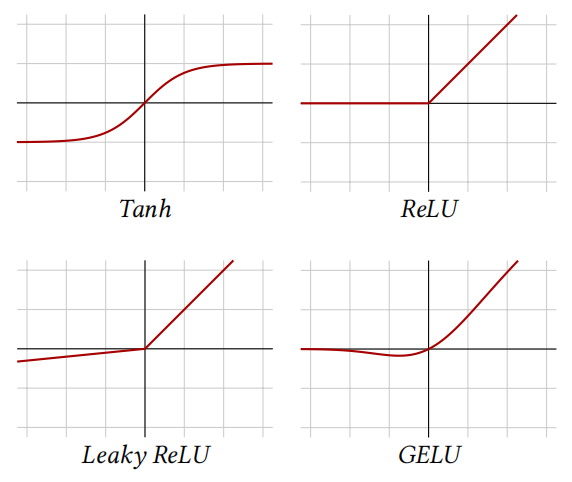
\includegraphics[width=0.9\textwidth]{fig/fig4.5.png}
    \caption[激活函数]{激活函数。}
    \label{fig4.5}
\end{figure}

在 ReLU 被普遍使用之前,标准激活函数是\keyterm{双曲正切函数}(\keyterm{Tanh},见图 \ref{fig4.5},左上),它在负半轴和正半轴都会以指数速度快速饱和,这加剧了梯度消失。

其他流行的激活函数遵循相同的思路,即保持正值不变压缩负值。\keyterm{Leaky ReLU} \citep{relu_hybrid_icml2013_final} 对负值应用一个小的正乘法因子(见图 \ref{fig4.5},左下):
$$
\text{leakyrelu}(x) = \begin{cases}
    ax &\text{如果}\; x < 0 \\
    \enspace x &\text{如果}\; x \ge 0
 \end{cases}
 $$
 而 \keyterm{GELU} \citep{arxiv-1606.08415} 是利用高斯分布的累积分布函数来定义的,即:
 \[\text{gelu}(x) = xP(Z \le x)\]
 其中 $Z \sim \mathcal{N} (0,1)$。它的行为大致类似于平滑的 ReLU(见图 \ref{fig4.5},右下)。

 激活函数的选择,特别是 ReLU 变体的选择,通常是由经验表现驱动的。

\section{池化}\label{sec4.4}

减少信号大小的一种经典策略是使用\keyterm{池化}操作,将多个激活合并为一个理想情况下能总结信息的激活。此类操作中最标准的是\keyterm{最大池化}层,它与卷积类似,可以在一维和二维中操作,并由\keyterm{内核大小}定义。

在其标准形式中,该层在空间大小等于内核大小的非重叠子张量上计算每个通道的最大激活。这些值存储在与输入具有相同通道数的结果张量中,并且其空间大小能被内核大小整除。与卷积一样,该算子具有三个\keyterm{元参数}:\keyterm{填充}、\keyterm{步长}和\keyterm{膨胀},默认情况下步长等于内核大小。遵循与卷积相同的公式(参见第 \ref{sec4.2} 节),较小的步长会产生较大的结果张量。

最大操作可以直观地解释为逻辑析取,或者,当它经过一系列通过计算局部分数来表示部件存在的\keyterm{卷积层}时,作为一种编码方式编码至少有一个部件实例存在。它牺牲了精确位置,从而使其不受局部变形的影响。

一个常见的替代方案是\keyterm{平均池化}层,它计算子张量上的平均值而不是最大值。这是一种线性操作,而最大池化则不是。

\begin{figure}
    \centering
    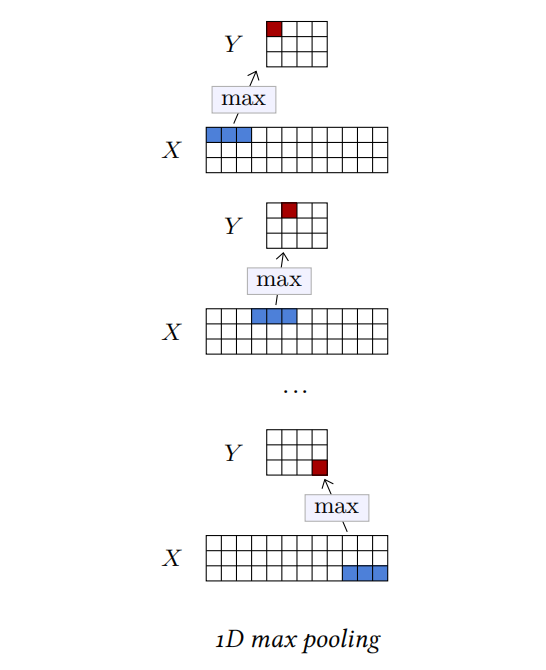
\includegraphics[width=0.9\textwidth]{fig/fig4.6.png}
    \caption[最大池化]{一维最大池化将 $D \times T$ 大小的张量 $X$ 作为输入,计算非重叠 $1 \times L$ 子张量(蓝色)的最大值,并将结果值(红色)存储在 $D \times (T / L)$ 大小的张量 $Y$ 中。}
    \label{fig4.6}
\end{figure}

\section{Dropout}\label{sec4.5}

某些层被专门设计用来促进训练或改进学学习得到的表示。

这类主要贡献之一是 \keyterm{Dropout} \citep{srivastava14a}。这种层没有可训练参数,但有一个元参数 $p$,并接受任意形状的张量作为输入。

通常在测试期间会关闭 Dropout,这种情况下其输出等于输入。当它处于激活状态时,它有概率 $p$ 独立地将输入张量的每个激活置为零,并且以 $\frac{1}{1-p}$ 因子重新缩放所有激活以保持期望值不变(见图 \ref{fig4.7}) 。

\begin{figure}
    \centering
    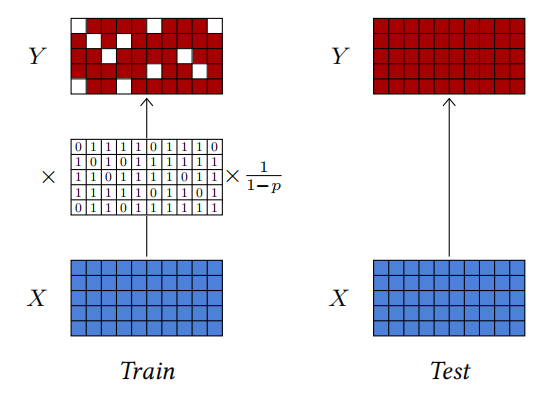
\includegraphics[width=0.9\textwidth]{fig/fig4.7.png}
    \caption[Dropout]{Dropout 可以处理任意形状的张量。在训练期间(左),它以概率 $p$ 将激活随机设置为零,并应用乘法因子来保持预期值不变。在测试期间(右),它保持所有激活不变。}
    \label{fig4.7}
\end{figure}

使用 Dropout 的动机在于促进有意义的单个激活,并阻止群体表征。由于一组 $k$ 个激活通过 Dropout 层保持完整的概率为 $(1-p)^k$,因此联合表征变得不可靠,从而使训练过程避免使用它们。Dropout 也可以被视为一种噪声注入,使训练更加稳健。

在处理图像和二维张量时,信号的短期相关性和由此产生的冗余抵消了 Dropout 的影响,因为可以从其邻居中推断出设置为零的激活。 因此,二维张量的 Dropout 将整个通道设置为零,而不是单个激活(见图 \ref{fig4.8})。

\begin{figure}
    \centering
    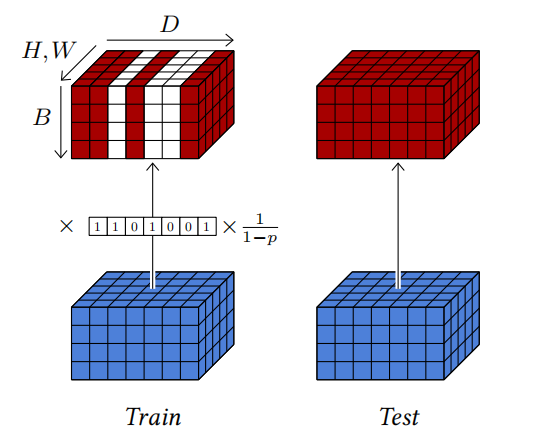
\includegraphics[width=0.9\textwidth]{fig/fig4.8.png}
    \caption[二维 Dropout]{诸如图像之类的二维信号通常表现出很强的短期相关性,并且可以从其邻居中推断出各个激活。这种冗余消除了标准非结构化 Dropout 的影响,因此二维张量的常用 Dropout 层会丢弃整个通道而不是单个值。}
    \label{fig4.8}
\end{figure}

尽管 Dropout 通常用于改进训练而在推理过程中处于非活动状态,但它可以在某些设置中用作随机化策略,例如,根据经验估计置信度分数 \citep{arxiv-1506.02142}。

\section{归一化层}\label{sec4.6}

在深度架构训练中,一类重要的操作是\keyterm{归一化层},它强制对一组激活函数的经验平均值和方差进行标准化。

这一类别的主要层是\keyterm{批量归一化} \citep{icml43442},它是唯一一个处理整批数据而不是单个样本的标准层。它由元参数 $D$ 和两组可训练标量参数 $\beta_1,\dots,\beta_D$ 和 $\gamma_1,\dots,\gamma_D$ 参数化。

给定一个由 $B$ 个 $D$ 维样本 $x_1,\dots,x_B$ 组成的批数据,它首先计算每个 D 分量的经验平均值 $\hat{m}_d$ 和方差 $\hat{v}_d$:
\begin{align*}
    \hat{m}_d &= \frac{1}{B}\sum_{b=1}^{B}x_{b,d} \\
    \hat{v}_d &= \frac{1}{B}\sum_{b=1}^{B}(x_{b,d}-\hat{m}_d)^2
\end{align*}
从中计算每个分量 $x_{b,d}$ 的归一化值 $z_{b,d}$,经验平均值为 $0$,方差为 $1$,并由此得出最终结果值 $y_{b,d}$,平均值为 $\beta_d$,标准差为 $\gamma_d$:
\begin{align*}
    \forall b, \quad z_{b,d} &= \frac{x_{b,d}-\hat{m}_d}{\sqrt{\hat{v}_d+\epsilon}}\\
    y_{b,d} &= \gamma_dz_{b,d}+\beta_d
\end{align*}
由于此标准化是跨批次定义的,因此仅在训练期间完成。在测试过程中,该层根据整个训练集上偏移平均值估计的 $m_d$ 和 $v_d$ 来转换各个样本,这可以归结为每个组件的固定仿射变换。

批量归一化背后的动机是避免网络早期层在训练期间的缩放变化影响到后续所有层,这些层随后需要相应地调整它们的可训练参数。尽管实际的作用机制可能比这一初衷更加复杂,但这种层显著地简化了深度模型的训练过程。

在二维张量的情况下,为了遵循卷积层处理所有位置的相似性原则,归一化是按通道进行的,覆盖所有二维位置,而 $\beta$ 和 $\gamma$ 仍然是 $D$ 维向量,因此缩放/偏移不依赖于二维位置。因此,如果待处理张量的形状为 $B \times D \times H \times W$,对于 $d = 1,\dots,D$,该层根据相应的 $B \times H \times W$ 切片计算 $(\hat{m}_d,\hat{v}_d)$,对其进行归一化。最后使用可训练参数 $\beta_d$ 和 $\gamma_d$ 缩放和偏移其分量。

\begin{figure}
    \centering
    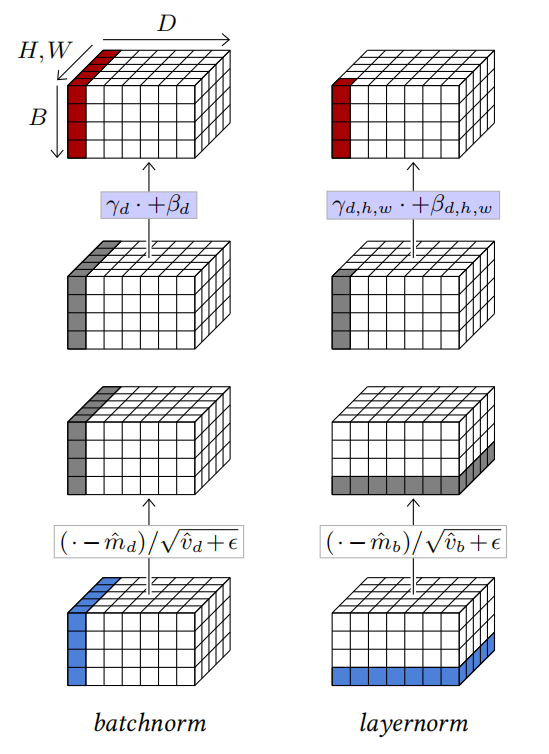
\includegraphics[width=0.9\textwidth]{fig/fig4.9.png}
    \caption[批量归一化]{批量归一化(左)对给定 $d$ 的每组激活的均值和方差进行归一化,并使用每个 $d$ 的学习参数缩放/偏移同一组激活。层归一化(右)对特定 $b$ 的每组激活进行归一化,并使用由相同索引的学习参数对给定 $d,h,w$ 的每组激活进行缩放/偏移。}
    \label{fig4.9}
\end{figure}

因此,给定一个 $B \times D$ 张量,批量归一化会在 $b$ 上对其进行归一化,并根据 $d$ 对其进行缩放/偏移,这可以通过 $\gamma$ 的逐元素乘积和与 $\beta$ 的求和来实现。给定 $B \times D \times H \times W$ 张量,它会根据 $b,h,w$ 进行归一化,并根据 $d$ 进行缩放/偏移(参见图 \ref{fig4.9},左图)。

这种方法可以根据这些维度进行泛化。例如,\keyterm{层归一化} \citep{arxiv-1607.06450} 计算单个样本所有分量的矩,并进行归一化,然后对各个分量分别进行缩放和偏移(参见图 \ref{fig4.9},右图)。因此,给定一个 $B \times D$ 的张量,它会根据 $d$ 进行归一化,并且根据相同的维度进行缩放/偏移。给定一个 $B \times D \times H \times W$ 的张量,它会根据 $d,h,w$ 进行归一化,并且根据同样的维度进行缩放/偏移。

\newpage

与批量归一化不同的是,由于层归一化单独处理每个样本,因此它在训练和测试期间的表现是相同的。

\section{跳跃连接}\label{sec4.7}

另一种缓解梯度消失问题并允许深层架构训练的技术是\keyterm{跳跃连接} \citep{arxiv-1411.4038, arxiv-1505.04597}。它本身并不是层,而是一种架构设计,在该设计中,某些层的输出会原样传输到模型中更深的其他层,绕过中间的处理。这个未经修改的信号可以与连接分支进入的层的输入进行连接或相加(参见图 \ref{fig4.10})。一种特殊类型的跳跃连接是\keyterm{残差连接},它通过求和来结合信号,并且通常只跳过几个层(参见图 \ref{fig4.10},右侧)。

这种设计最理想的特性是,确保即使在某个阶段出现了梯度消除的处理情况,梯度仍然能够通过跳过连接进行传播。特别是残差连接,它允许构建多达数百层的深度模型和关键模型,例如计算机视觉中的\keyterm{残差网络} \citep{arxiv-1512.03385}(详见 \ref{sec5.2} 节)和自然语言处理中的 \keyterm{Transformers} \citep{arxiv-1706.03762}(详见 \ref{sec5.3} 节),完全都是由带有残差连接的层块组成的。

\newpage

\begin{figure}
    \centering
    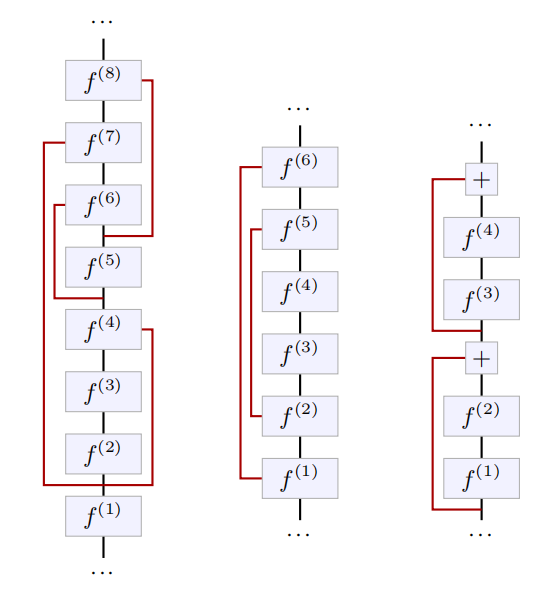
\includegraphics[width=0.9\textwidth]{fig/fig4.10.png}
    \caption[跳跃连接]{在这张图中,用红色突出显示的跳过连接将信号不变地跨越多个层传递。一些架构(中间)会缩小再放大表征的尺寸,以便在多个尺度上操作,它们采用跳过连接将网络早期部分的输出送至后续在相同尺度上操作的层 \citep{arxiv-1411.4038, arxiv-1505.04597}。而残差连接(右侧)是一种特殊的跳过连接,它将原始信号与转换后的信号相加,通常最多绕过几个层 \citep{arxiv-1512.03385}。}
    \label{fig4.10}
\end{figure}

跳跃连接还可以促进模型的多尺度推理,通过连接具有兼容大小的层,在重新放大信号大小之前减小信号大小,例如用于\keyterm{语义分割}(详见 \ref{sec6.4} 节)。在残差连接的情况下,它们还可以通过简化学习任务,使其变为寻找一个增量改进而不是完全更新,从而促进学习。

\section{注意力层}\label{sec4.8}

在许多应用中,需要一种操作能够结合张量中相隔较远位置的局部信息。例如,在\keyterm{图像合成}中为了生成连贯且真实的细节,或者在\keyterm{自然语言处理}中为了做出语法或语义决策,需要结合段落中不同位置的单词。

\keyterm{全连接层}无法处理高维信号,也无法处理可变大小的信号,并且\keyterm{卷积层}无法快速传播信息。例如,通过在大空间区域上求平均值来聚合卷积结果的策略会受到将多个信号混合到有限数量维度的困扰。

\keyterm{注意力层}通过计算结果张量的每个分量到输入张量的每个分量的注意力得分来专门解决这个问题,没有局部性约束,并相应地对整个张量的特征进行平均 \citep{arxiv-1706.03762}。

尽管注意力层比其他层复杂得多,但它已然成为许多最新模型的标准元素。特别是,它是 \keyterm{Transformer} 的关键构建块,Transformer 是\keyterm{大语言模型}的主导架构。参见 \ref{sec5.3} 和 \ref{sec7.1} 节。

\subsubsection*{注意力算子}

给定
\begin{itemize}
    \item $Q$ 为具有 $N^Q \times D^{QK}$ 大小的\keyterm{查询}张量
    \item $K$ 为具有 $N^{KV} \times D^{QK}$ 大小的\keyterm{键}张量
    \item $V$ 为具有 $N^{KV} \times D^V$ 大小的\keyterm{值}张量
\end{itemize}
\keyterm{注意力算子}计算 $N^Q \times D^V$ 维张量
\[Y = \text{att}(K,Q,V)\]
为此,它首先为每个查询索引 $q$ 和每个键索引 $k$ 计算一个注意力得分 $A_{q,k}$,作为查询 $Q_q$ 和键点积的 \keyterm{softargmax}:
\begin{equation}
    A_{q,k} = \frac{\exp\Big(\frac{1}{\sqrt{D^{QK}}}Q_q \cdot K_k\Big)}{\sum_{l}^{}\exp\Big(\frac{1}{\sqrt{D^{QK}}}Q_q \cdot K_l\Big)} \label{eq4.1}
\end{equation}
其中缩放因子 $\frac{1}{\sqrt{D^{QK}}}$ 即使对于较大的 $D^{QK}$ 也能保持值的范围大致不变。

然后,根据注意力得分对值进行加权平均,为每个查询计算出一个检索值(参见图 \ref{fig4.11}):
\begin{equation}
    Y_q = \sum_{K}^{}A_{q,k}V_k \label{eq4.2}
\end{equation}

\begin{figure}
    \centering
    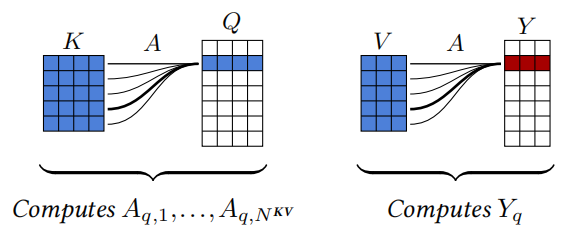
\includegraphics[width=0.9\textwidth]{fig/fig4.11.png}
    \caption[注意力算子解析]{注意力算子可以解释为将每个查询 $Q_q$ 与所有键 $K_1, \dots ,K_{N^{KV}}$ 进行匹配,以获得归一化注意力得分 $A_{q,1}, \dots ,A_{q,N^{KV}}$(见左图和公式 \ref{eq4.1}),然后将值 $V_1, \dots ,V_{N^{KV}}$ 根据这些得分进行加权平均,计算出结果 $Y_q$(见右图和公式 \ref{eq4.2})。}
    \label{fig4.11}
\end{figure}

因此,如果查询 $Q_n$ 与某个键 $K_m$ 的匹配程度远远高于所有其他键,则相应的注意力得分 $A_{n,m}$ 将接近于 $1$,而检索到的值 $Y_n$ 将是与该键关联的值 $V_m$。但是,如果它与多个键匹配程度相当,则 $Y_n$ 将是这些相关键关联值的平均值。

这可以实现为
\[\text{att}(Q,K,V) = \underbrace{\text{softargmax}\bigg(\frac{QK^T}{\sqrt{D^{QK}}}\bigg)V}_{A}\]

\begin{figure}
    \centering
    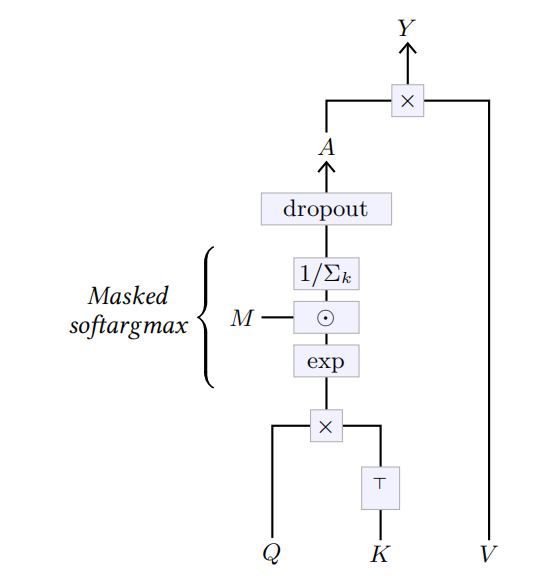
\includegraphics[width=0.9\textwidth]{fig/fig4.12.png}
    \caption[完全注意力算子]{注意力算子 $Y = \text{att}(Q,K,V)$ 首先计算注意力矩阵 $A$ 作为 $QK^T$ 的每个查询的 softargmax,它可以在归一化之前被常量矩阵 $M$ 屏蔽。该注意力矩阵在乘以 $V$ 以获得结果 $Y$ 之前先经过一个 dropout 层。通过将 $M$ 对角线下方全置为 $1$,对角线上方全置为 $0$,可以使该算子具有\keyterm{因果性}。}
    \label{fig4.12}
\end{figure}

如图 \ref{fig4.12} 所示,该操作通常以两种方式扩展。首先,可以在 softargmax 归一化之前将注意力矩阵乘以布尔矩阵 $M$ 来屏蔽注意力矩阵。例如,这允许通过取 $M$ 对角线以下全为 $1$ 而对角线以上全为 $0$ 来使算子具有\keyterm{因果性},从而防止 $Y_q$ 依赖于索引 $k$ 大于 $q$ 的键和值。其次,注意力矩阵在乘以 $V$ 之前由 \keyterm{dropout 层}(参见 \ref{sec4.5} 节)进行处理,从而在训练期间提供通常的好处。

\subsubsection*{多头注意力层}

\begin{figure}
    \centering
    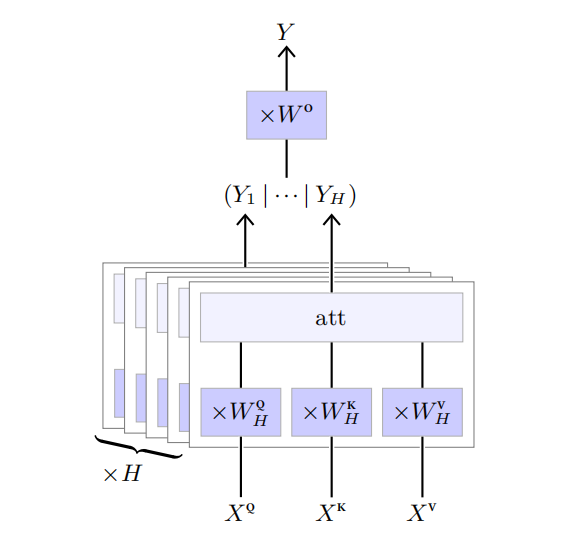
\includegraphics[width=0.9\textwidth]{fig/fig4.13.png}
    \caption[多头注意力层]{多头注意力层对其每一个头 $h = 1,\dots,H$,都对输入序列 $X^Q, X^K, X^V$ 的各个元素施加一个参数化的线性变换,得到将由注意力算子处理以计算 $Y_h$ 的序列 $Q,K,V$。这 $H$ 个序列沿特征连接在一起,个别元素通过最后一个线性算子,得到最终的结果序列 $Y$。}
    \label{fig4.13}
\end{figure}

这个无参数注意力算子是图 \ref{fig4.13} 所示的多头注意力层中的关键元素。该层的结构由几个元参数定义:头的数量 $H$ 以及三组 $H$ 个可训练权重矩阵
\begin{itemize}
    \item $W^Q$ 尺寸为 $H \times D \times D^{QK}$
    \item $W^K$ 尺寸为 $H \times D \times D^{QK}$
    \item $W^V$ 尺寸为 $H \times D \times D^V$
\end{itemize}
分别计算输入中的查询、键和值,以及最终的权重矩阵 $W^O$,其大小为 $HD^V \times D$,用于聚合每个头的结果。

它以三个序列
\begin{itemize}
    \item $X^Q$ 尺寸为 $N^Q \times D$
    \item $X^K$ 尺寸为 $N^{KV} \times D$
    \item $X^V$ 尺寸为 $N^{KV} \times D$
\end{itemize}
作为输入,并从中进行计算,对于 $h = 1,\dots,H$,
\[Y_h = \text{att}\Big(X^QW_h^Q, X^KW_h^K, X^VW_h^V\Big)\]
该序列 $Y_1,\dots,Y_H$ 沿特征维度连接,并将所得序列的每个单独元素乘以 $W^O$ 以获得最终结果:
\[Y = \Big(Y_1 \mid \dots \mid Y_H\Big)W^O\]
正如我们将在 \ref{sec5.3} 节和图 \ref{fig5.6} 中看到的,该层用于构建两个模型子结构:\keyterm{自注意力块}(其中三个输入序列 $X^Q$、$X^K$ 和 $X^V$ 相同)和\keyterm{交叉注意力块}(其中 $X^K$ 和 $X^V$ 相同)。

值得注意的是,注意力算子,以及当没有屏蔽时的多头注意力层,对键和值的排列是不变的,并且与查询的排列\keyterm{等价},因为它会以类似的方式排列结果张量。

\section{Token 嵌入}\label{sec4.9}

在许多情况下,我们需要将离散 Token 转换为向量。这可以通过\keyterm{嵌入层}来完成,该层由一个直接将整数映射到向量的查找表组成。

嵌入层由两个\keyterm{元参数}定义:可能的 Token 值的数量 $N$,以及输出向量的维度 $D$,还一个 $N \times D$ 大小的可训练权重矩阵 $M$。

给定维度为 $D_1 \times \dots \times D_K$ 的整数张量 $X$ 和 ${0, \dots ,N -1}$ 中的值作为输入,嵌入层返回维度为 $D_1 \times \dots \times D_K \times D$ 的实值张量 $Y$,具体公式如下:
\begin{align*}
    \forall d_1, \dots, d_K,& \\
    Y[d&_1, \dots, d_K] = M[X[d_1, \dots, d_K]]
\end{align*}

\section{位置编码}\label{sec4.10}

虽然\keyterm{全连接层}的处理既特定于输入张量中特征的位置,也特定于输出张量中激活结果的位置,但\keyterm{卷积层}和\keyterm{多头注意力层}并不关心张量中的绝对位置。这是它们强大\keyterm{不变性}和\keyterm{归纳偏置}的关键,对于处理固定信号非常有益。

然而,在某些需要访问绝对位置才能进行恰当处理的情况下,这可能是个问题。例如,在图像合成中,场景的统计特性并不完全固定,或者在自然语言处理中,单词的相对位置强烈地调节了句子的含义。

解决这个问题的标准方法是在每个位置向特征表示中添加或连接一个\keyterm{位置编码},这是一个依赖于张量中位置的特征向量。这种位置编码可以像其他层参数一样被学习,或者通过分析来定义。

例如,在原始 \keyterm{Transformer} 模型中,对于一系列 $D$ 维向量,\cite{arxiv-1706.03762} 将序列索引的编码添加为一系列不同频率的正弦和余弦:
\begin{align*}
    \text{pos-enc}[t,d] &= \\
    &\begin{cases}
        \sin\Big(\frac{t}{T^{d/D}}\Big) &\text{如果}\; d \in 2\mathbb{N}\\
        \cos\Big(\frac{t}{T^{(d-1)/D}}\Big) &\text{否则}
    \end{cases}
\end{align*}
其中 $T= 10^4$